%\Large\mathphyssubsubsec{Lehramt Informatik}\normalfont\small
\section{50\%-Bachelor Informatik (Lehramt)}
\sidebar{
	\centering
	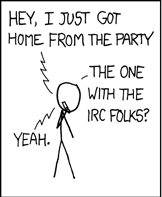
\includegraphics[width=3.5cm]{bilder/xkcd_responsible_behaviour_1.png}\\\vspace{10mm}
	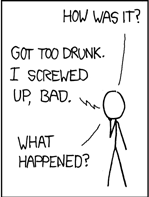
\includegraphics[width=3.5cm]{bilder/xkcd_responsible_behaviour_2.png}\\\vspace{10mm}
	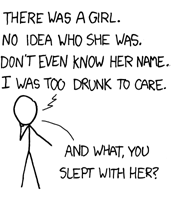
\includegraphics[width=3.5cm]{bilder/xkcd_responsible_behaviour_3.png}\\\vspace{10mm}
	
\includegraphics[width=3.1cm]{bilder/xkcd_responsible_behaviour_4.png}
}

Wenn ihr den 50\%-Bachelor Informatik studiert, sind zwei Fälle zu unterscheiden: Ihr hört in
eurem zweiten Fach Mathematik Veranstaltungen oder ihr tut es nicht. Diese
Unterscheidung rührt daher, dass ihr in der Informatik auf jeden Fall etwas
Mathematik können solltet, wenn ihr in eurem anderen fach Mathe hört habt ihr das aber
schon da abgedeckt und ihr könnt euch in dieser Hälfte eures Bachelors ganz auf die Informatik konzentrieren.

Auf jeden Fall Hört ihr im Ersten Semester \hyperref[info1]{„Einführung in die Praktische Informatik“ (Info 1)},
die ist Wichtig da es eure Orientierungsprüfung in Informatik ist, und den Programmierkurs.
Im zweiten Semester solltet ihr dann in Informatik die „Einführung in die Theoretische Informatik“
\footnote{„Theo“ kann zu verwirungen mit Physikern führen da diese das als Theoretische Physik verstehen}
und „Algorithmen und Datenstrukturen“ (AlDa) hören. Im Dritten Semester macht sich der Unterschied 
ob ihr in eurem Zweiten Fach Mathe hört oder nicht da ihr hier „Mathematik für Informatiker 1“ (MafIn 1) sollt,
wenn ihr aber bereits andere Mathe Veranstaltungen Bestanden habt könnt ihr beim Prüfungsausschuss beantragen
das ihr statt dessen ein weiteres Info Modul, aus dem Bereich der Wahlpflicht Veranstaltungen, hören könnt.
Ausserdem ist vorgesehen das ihr im Dritten Semester die „Einführung in die Technische Informatik“
(ITE oder Technische Info)\footnote{dafür hat leider noch niemand eine schön Abkürzung gefunden}.
Im Vierten und Fünften Semester stehen dann „Betriebssysteme und Netzwerke“ (BeNe),
„Software Engineering“ (ISW) und ein Proseminar. Im Sexten Semester müsst ihr dann neben der Bachelorarbeit,
die ihr in einem eurer beiden Fächer schreibt, noch „Datenbanken 1“ (IDB1) hören.
Zusätzlich müsst ihr noch ein Anfängerpraktikum und ein Seminar hören.
Da ihr vermutlich nach dem Bachelor noch den „Master of Education“ machen wollt müsst ihr 
das Proseminar und das Anfängerpraktikum im Themenbereich „Informatik und Gesellschaft“ (IuG)
machen. Da im Seminar und Proseminar und Seminar schon LP als „Fachübergreifende Kompetenzen“ (FÜK)
vergeben werden habt ihr noch 4 LP die ihr mit einer FÜK Veranstaltung eurer Wahl holen könnt.

Ihr solltet euch bei jeder Veranstaltung genau darüber informieren,
was ihr benötigt um zur Prüfung zugelassen zu werden (z.B. 50\% auf
den Übungszetteln) und was genau \emph{eine} Prüfung beinhaltet
(z.\,B.\ Bestehen von einer von zwei Klausuren). Insbesondere der
letzte Teil ist wichtig, denn ihr könnt Prüfungen grundsätzlich
zweimal versuchen. Je nach Veranstaltung und Dozent/in \emph{können}
zwei Klausuren als eine Prüfung zählen, müssen aber nicht -- dann
würde jede geschriebene Klausur als ein Prüfungsversuch gelten. Wenn
ihr aus Gründen, die ihr nicht zu verantworten habt (wie krank sein),
nicht an einer \emph{Prüfung} teilnehmen konntet, erhöhen sich
entsprechend eure Versuche. Wenn ihr alle \emph{Klausur}termine
verpasst habt, kann die Klausur auch durch eine mündliche Prüfung
ersetzt werden. Sollte das bei euch mal der Fall sein, fragt ihr
jedoch am besten den/die Dozent/in.

Leider habt ihr nur sehr wenig Wahlmöglichkeiten da die meisten Veranstaltungen verpflichtend sind.
Einen Anhaltspunkt für die Planung eures Studiums können die Musterstudienpläne in eurer
Prüfungsordnung sein, die „nach Vorgabe“ erstellt wurden -- d.\,h.\
ca.\ 15 Leistungspunkte pro Semester -- gleichzeitig aber versucht
wurde, die Veranstaltungen möglichst sinnvoll anzuordnen.
